% 需求分析
\chapter{需求分析}
\section{功能需求}
	\subsection{功能划分}
		\begin{itemize}
			\item 添加数据
			\item 修改数据
			\item 数据与数据库同步
		\end{itemize}
	\subsection{功能描述}
		\begin{itemize}
			\item 添加数据: 友好的添加数据。
			\item 删除数据: 友好的删除数据。
			\item 数据与数据库同步: 及时与数据库数据同步,不会造成数据丢失。
		\end{itemize}
\section{运行需求}
	\subsection{用户界面}
		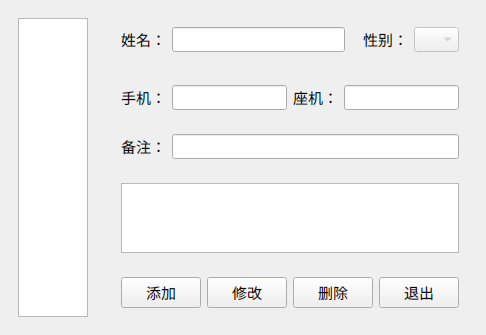
\includegraphics[scale=0.6]{ui.png}
